\subsection{Validation}


 Validation of models is important to ascertain that the output is accurate. However, it should be noted that these long-term simulations are not predictions of the future, rather possible outcomes based upon certain assumptions. Jager posits that a certain outcome or development path, captured by empirical data, might have developed in a completely different direction due to chance \cite{Jager2006a}. However the processes that emerge from a model should be realistic and in keeping with expected behaviour \cite{Jager2006}.

We begin by comparing the price duration curve in the year 2018. Figure \ref{fig:price_duration_curve} shows the N2EX Day Ahead Auction Prices of the UK \cite{nordpool_2019}, the stochastic simulated electricity prices, and the non-stochastic electricity price throughout the year 2018. The N2EX Day Ahead Market is a day ahead market run by Nord Pool AS. Nord Pool AS runs the largest market for electrical energy in Europe, measured in volume traded and in market share \cite{nordpool_2019}.


\begin{figure}
	\begin{center}
		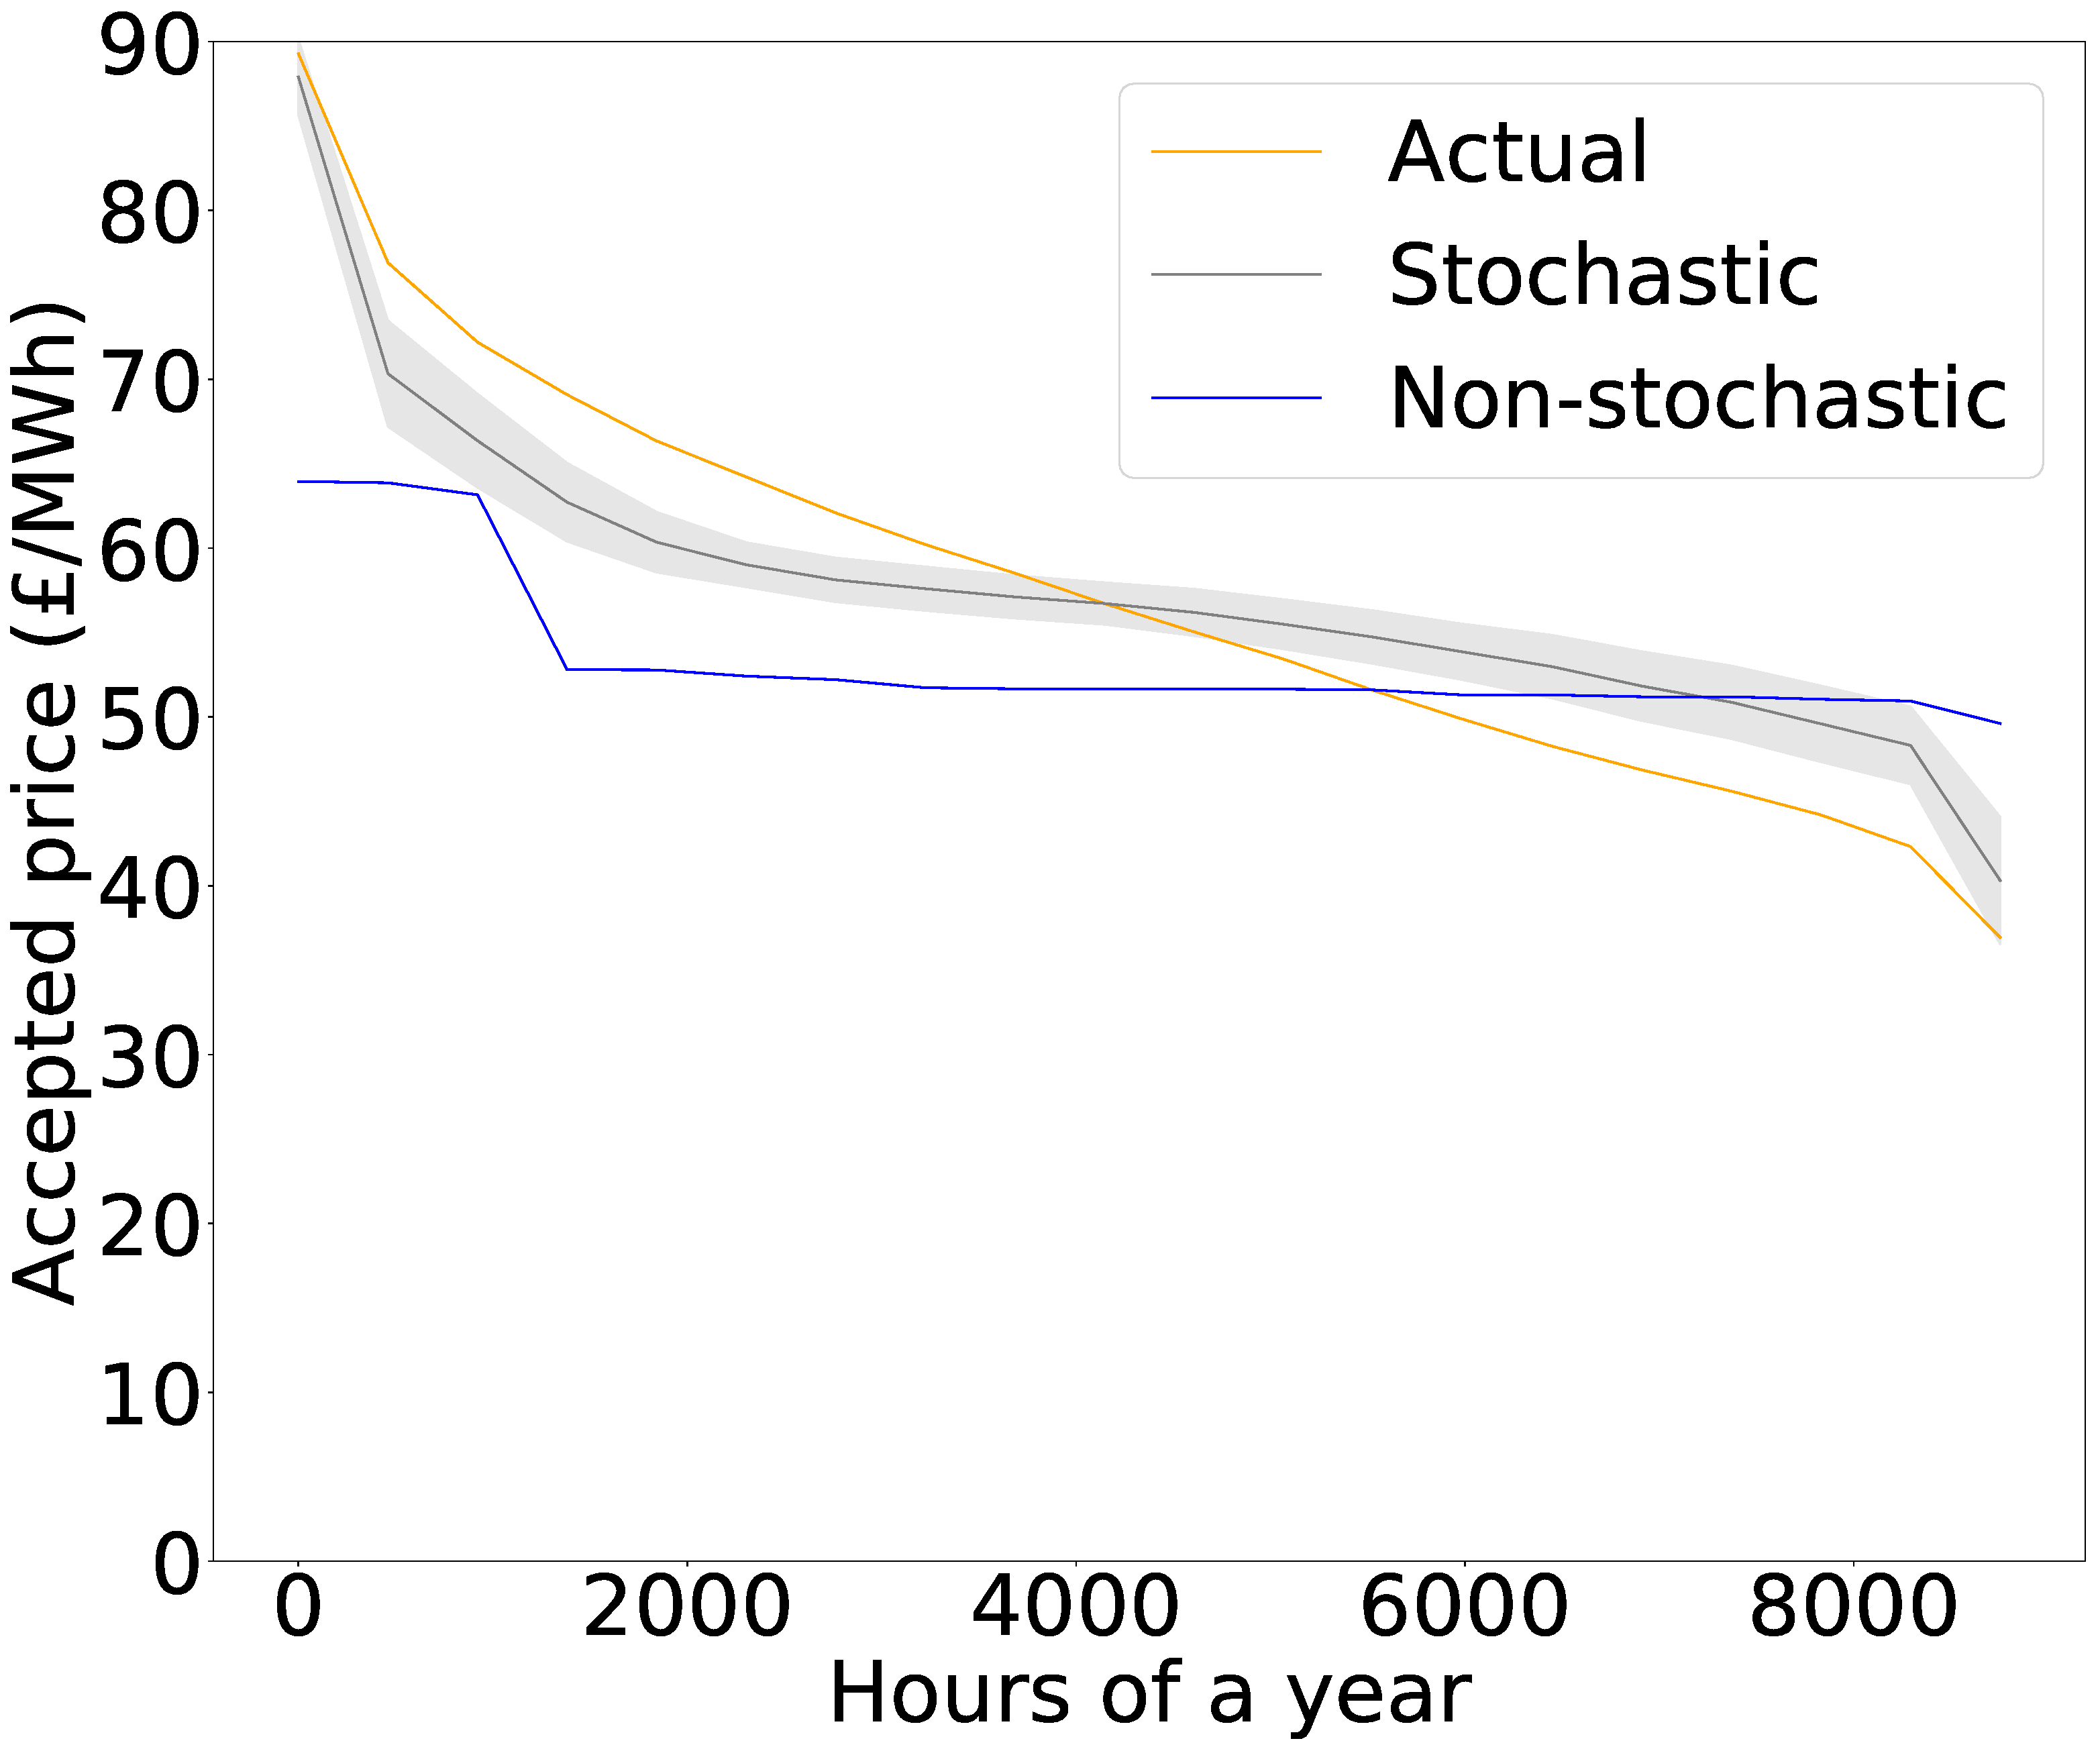
\includegraphics[width=0.35\textwidth]{figures/load_price_duration_curve_comparison.pdf}
		\caption{Price duration curve which compares real electricity prices to those paid in ElecSIM with and without stochasticity (2018).}
		\label{fig:price_duration_curve}
	\end{center}
\end{figure}
\begin{table}
	\centering
	\csvautobooktabular{tables/validation/initialisation_run_validation.csv}
	\caption{Validation performance metrics.}
	\label{table:validation_metrics}
\end{table}

We ran the initialisation of the model 40 times to capture the price variance. Outliers were removed as on a small number of occasions large jumps in prices at peak demand occurred which deviated from the mean. We did this, as although this does occur in real life, it occurs at a smaller fraction of the time than 5\% of the year (modelled LDC), therefore the results would be unreasonably skewed for the highest demand segment. 

Figure \ref{fig:price_duration_curve} demonstrates very little variance in the non-stochastic case. This is due to the fact that combined cycle gas turbines (CCGTs) set the spot price. These CCGTs have little variance between one another as they were calibrated using the same dataset. By adding stochasticity of fuel prices and operation and maintenance prices, a curve that more closely resembles the actual data occurs. The stochastic curve, however, does not perfectly fit the real data, which may be due to higher variance in fuel prices and historical differences in operation and maintenance costs between power plants. One method of improving this would be fitting the data used to parametrise to the curve.

Table \ref{table:validation_metrics} shows performance metrics of the stochastic and non-stochastic runs versus the actual price duration curve . The stochastic implementation, improves the mean absolute error (MAE) of the non-stochastic case by $52.5\%$.

By observing the processes that emerge from the long-term scenarios, we can see that carbon price and investment in renewable generation are positively correlated, as would be expected.

The highest NPV calculations were for onshore wind and CCGT plants. This is realistic for the United Kingdom, where subsidies are required for other forms of generation such as coal and nuclear.

\subsection{Performance}

 We used Microsoft Azure Public Cloud. Utilising two virtual machines of 64 vCPU's each (D64 v3), which are built using Intel Broadwell E5-2673 v4 2.3GHz processors, and the Intel Haswell 2.4 GHz E5-2673 v3. They have a total of 256GB of memory and use a Linux operating system. The total disk size of ElecSIM is 5.8MB. The memory used for a 10 year run has a median of 57.1MB.




Figure \ref{fig:timingplot} shows the running time for ElecSIM with varying installed capacity. We varied demand between 2GW and 320GW to see the effect of different sized countries on running time. The makeup of the electricity mix was achieve through stratified sampling of the UK electricity mix. The results show a linear time complexity. 

\begin{figure}
	\centering
	\includegraphics[width=0.85\linewidth]{figures/timing_plot}
	\caption{Run times of different sized countries.}
	\label{fig:timingplot}
\end{figure}

%\begin{itemize}
%	\item Validation of model 
%	\begin{itemize}
%		\item Compare price duration curve
%		\item Compare power plant costs and NPV calculations
%		\item Look number of steps ahead to compare electricity mix and compare to actual (cross-validation)
%	\end{itemize} 
%	\item Performance metrics - Comparison with EMLab, PowerACE (15 minute run time)
%	\begin{itemize}
%		\item Memory, disk size, runtime
%		\item Increase in time complexity with additional data.
%	\end{itemize}
%\end{itemize}
